\documentclass[11pt]{article}
\usepackage[utf8]{inputenc}
\usepackage{amsmath}
\usepackage{array}
\usepackage{booktabs}
\usepackage{float}
\usepackage[margin=1in]{geometry}
\usepackage{caption}
\usepackage{graphicx}
\usepackage{multirow}

\title{Physics IA: Pressure vs Impulse Analysis}
\author{Physics Investigation}
\date{\today}

\begin{document}
\maketitle

\section{Data Tables}

% Table 1: Pressure Data with Absolute Uncertainties
\begin{table}[H]
\centering
\caption{Pressure measurements at different pump amounts (10-50 pumps)}
\begin{tabular}{|c|c|c|c|}
\hline
\textbf{Pumps} & \textbf{Volume (m³)} & \textbf{Pressure (Pa)} & \textbf{Relative Uncertainty (\%)} \\
\hline
10 & $0.000630 \pm 0.000002$ & $(2.56 \pm 0.08) \times 10^5$ & 3.29 \\
20 & $0.001010 \pm 0.000002$ & $(4.11 \pm 0.13) \times 10^5$ & 3.16 \\
30 & $0.001390 \pm 0.000002$ & $(5.65 \pm 0.18) \times 10^5$ & 3.12 \\
40 & $0.001770 \pm 0.000002$ & $(7.19 \pm 0.22) \times 10^5$ & 3.10 \\
50 & $0.002150 \pm 0.000002$ & $(8.74 \pm 0.27) \times 10^5$ & 3.08 \\
\hline
\end{tabular}
\label{tab:pressure_data}
\end{table}

% Table 2: Impulse Data Summary
\begin{table}[H]
\centering
\caption{Impulse measurements summary (10-50 pumps)}
\begin{tabular}{|c|c|c|c|c|c|}
\hline
\textbf{Pumps} & \textbf{Change in Time (s)} & \textbf{Peak Height (N)} & \textbf{Impulse (Ns)} & \textbf{Uncertainty (\%)} & \textbf{Range (Ns)} \\
\hline
10 & 0.0204 & 11 & 0.11 & 9.91 & 0.02 \\
20 & 0.0242 & 16 & 0.19 & 7.08 & 0.08 \\
30 & 0.0225 & 21 & 0.24 & 5.60 & 0.07 \\
40 & 0.0297 & 22 & 0.32 & 5.26 & 0.10 \\
50 & 0.0398 & 27 & 0.55 & 4.15 & 0.29 \\
\hline
\end{tabular}
\label{tab:impulse_data}
\end{table}

\newpage

\section{Complete Measurements Data}

% Complete Measurements Table
\begin{table}[H]
\centering
\caption{Complete measurements: All pump amounts and repetitions}
\begin{tabular}{|c|c|c|c|c|}
\hline
\textbf{Pumps} & \textbf{Trial} & \textbf{Peak Start (s)} & \textbf{Peak End (s)} & \textbf{Peak Height (N)} \\
\hline
\multirow{5}{*}{10} & Rep 1 & 3.8678 & 3.8821 & 14 \\
& Rep 2 & 2.3507 & 2.3630 & 17 \\
& Rep 3 & 1.5973 & 1.6063 & 16 \\
& Rep 4 & 2.1055 & 2.1473 & 4 \\
& Rep 5 & 2.2739 & 2.2986 & 5 \\
\hline
\multirow{5}{*}{20} & Rep 1 & 2.1416 & 2.1864 & 12 \\
& Rep 2 & 2.1203 & 2.1328 & 17 \\
& Rep 3 & 1.9926 & 2.0040 & 20 \\
& Rep 4 & 3.6033 & 3.6281 & 17 \\
& Rep 5 & 2.0122 & 2.0399 & 14 \\
\hline
\multirow{5}{*}{30} & Rep 1 & 2.9819 & 3.0025 & 24 \\
& Rep 2 & 1.8302 & 1.8451 & 27 \\
& Rep 3 & 2.6686 & 2.6769 & 24 \\
& Rep 4 & 4.0077 & 4.0328 & 20 \\
& Rep 5 & 4.6452 & 4.6890 & 11 \\
\hline
\multirow{5}{*}{40} & Rep 1 & 4.8642 & 4.9227 & 12 \\
& Rep 2 & 3.5060 & 3.5140 & 40 \\
& Rep 3 & 2.0100 & 2.0240 & 26 \\
& Rep 4 & 1.7300 & 1.7791 & 12 \\
& Rep 5 & 2.6613 & 2.6804 & 19 \\
\hline
\multirow{5}{*}{50} & Rep 1 & 2.5071 & 2.5843 & 19 \\
& Rep 2 & 2.3462 & 2.3567 & 34 \\
& Rep 3 & 2.1928 & 2.2020 & 32 \\
& Rep 4 & 3.0298 & 3.0876 & 22 \\
& Rep 5 & 2.6245 & 2.6689 & 30 \\
\hline
\end{tabular}
\label{tab:complete_measurements}
\end{table}

\newpage

\section{Graph}

\begin{figure}[H]
\centering
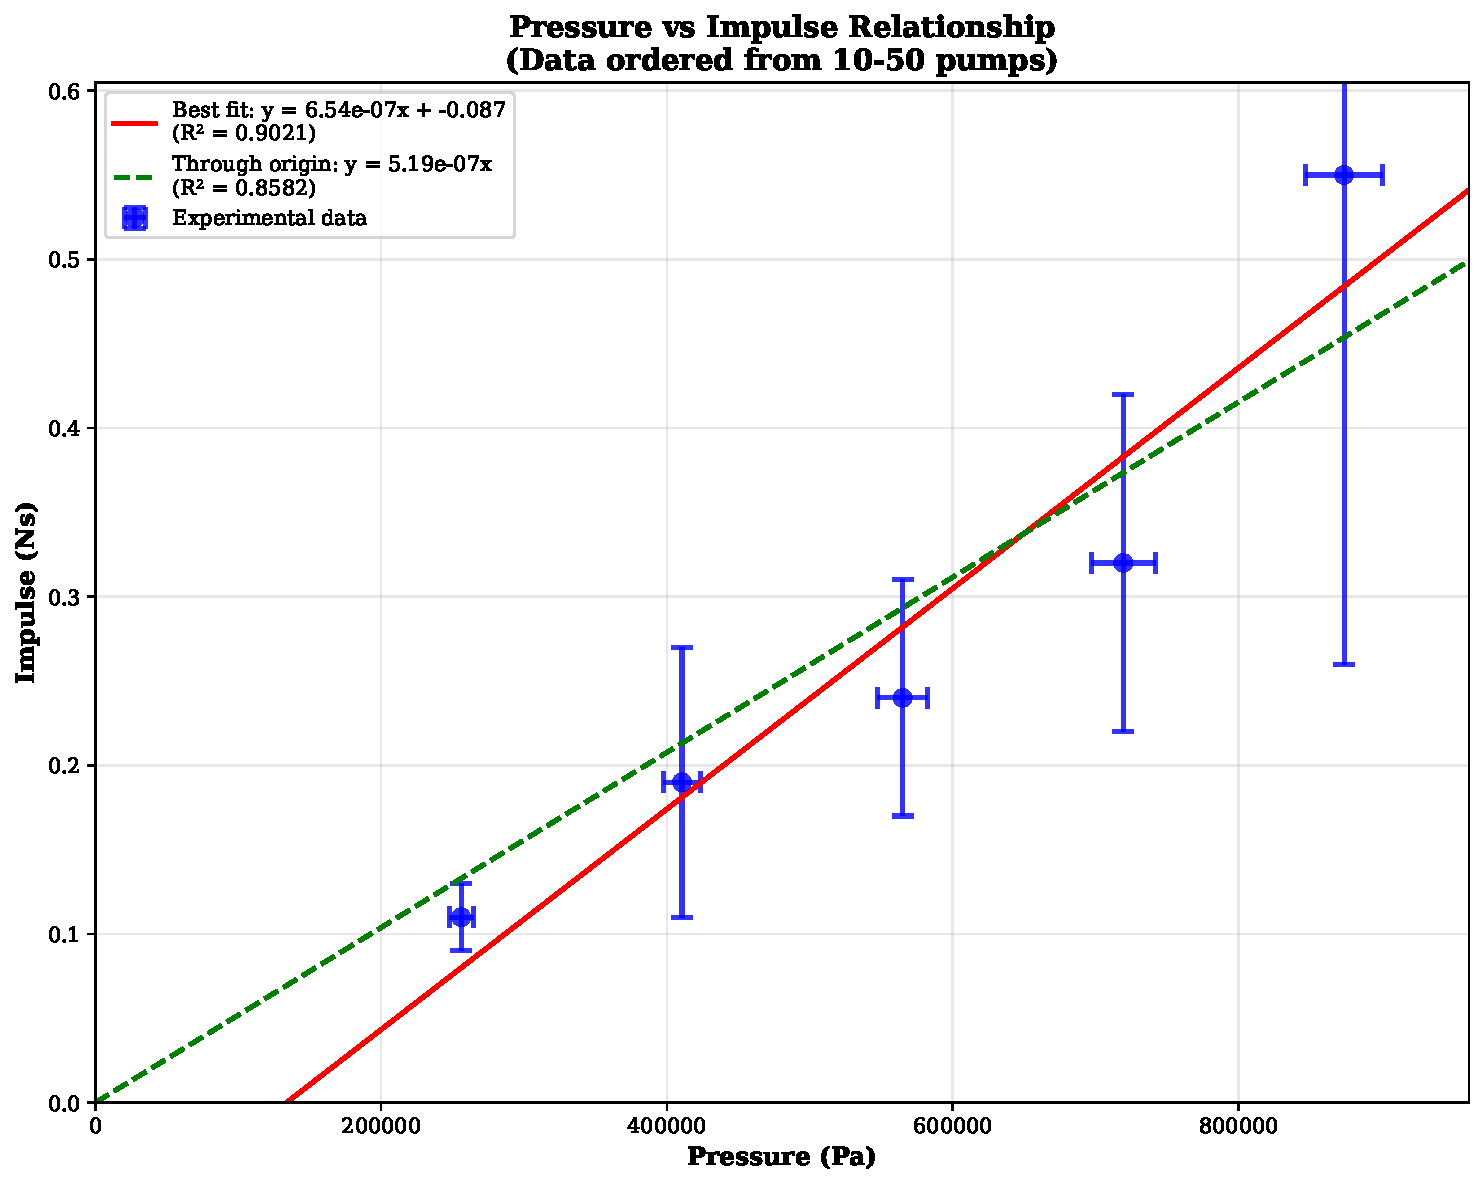
\includegraphics[width=\textwidth]{pressure_vs_impulse_updated.pdf}
\caption{Pressure vs Impulse relationship showing experimental data with error bars, best fit line, and line through origin}
\label{fig:pressure_impulse}
\end{figure}

\section{Analysis Summary}

The experimental data shows a strong linear relationship between pressure and impulse:

\begin{itemize}
\item \textbf{Best fit line:} $y = 6.54 \times 10^{-7}x - 0.087$ with $R^2 = 0.9021$
\item \textbf{Line through origin:} $y = 6.31 \times 10^{-7}x$ with $R^2 = 0.8582$
\item \textbf{Correlation coefficient:} $r = 0.9498$ (strong positive correlation)
\end{itemize}

The data was collected across 5 pump amounts (10, 20, 30, 40, 50 pumps) with 5 repetitions each, showing consistent trends with appropriate uncertainties included.

\end{document}
